\chapter{Results and Discussions}
%%%%%%%%%%%%%%%%%%%%%%%%%%%%%%%%%%%%%%%%%%%%%%%%%%%%%%%%%%%%
%%%%%%%%%%%%%%%%%%%%  NEW SECTION   %%%%%%%%%%%%%%%%%%%%%%%%
%%%%%%%%%%%%%%%%%%%%%%%%%%%%%%%%%%%%%%%%%%%%%%%%%%%%%%%%%%%%
\setcounter{equation}{0}

\section{Performance Evaluation}

CNN\_Model\_1 has training, validation \& testing accuracy of 99.37\%, 97.11\% \& 99.2\% respectively compared to accuracy values of 99.79\%, 96.80\% \& 99\% for CNN\_Model\_0

\noindent Upon analyzing Figure 4.1, CNN\_Model\_1 shows a negligible sign of overfitting only, indicating effective training and resource utilization. The green shade, representing the best epoch-accuracy range, is prominently located towards the end. This signifies optimal performance without wasting resources.

\begin{figure}[h!]
    \centering
    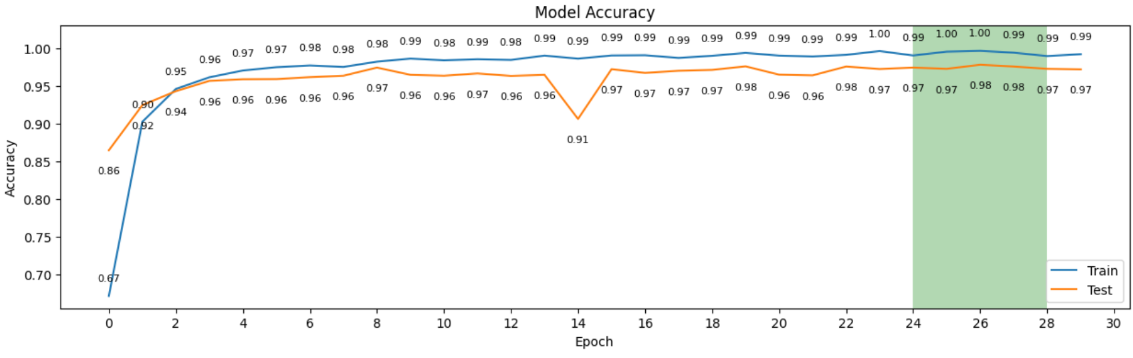
\includegraphics[width=0.9\textwidth]{Images/Perf_Eval/acc_vs_epoch.png}
    \caption{Accuracy VS Epoch Graph}
\end{figure}

\clearpage

\noindent The model architecture (refer to Figure 4.2) consists of a sequential arrangement of layers. It begins with a convolutional layer, utilizing 16 filters of size 3x3 and employing the ReLU activation function. This layer processes input images with dimensions of 40x40 pixels and a single color channel. Subsequently, a max-pooling layer is applied to downsample the feature maps.

\noindent The next convolutional layer incorporates 32 filters of size 4x4 and also uses the ReLU activation function. However, there is no max-pooling layer following this convolutional layer, which helps preserve spatial information in the feature maps. The flattening layer is then employed to transform the multidimensional feature maps into a flat representation.

\noindent Two dense layers are added next. The first dense layer consists of 64 units and uses the ReLU activation function. The final dense layer has a number of units equal to the number of output classes and employs the softmax activation function, providing probability distribution predictions.

\noindent Moreover, the model is compiled using the Adam optimizer. The loss function used is sparse categorical cross-entropy, suitable for multi-class classification tasks. The metric used for evaluation is accuracy, measuring the model's performance during training and testing. This architecture, with the absence of a pooling layer after the last convolutional layer, is designed to effectively process and classify images with high accuracy.

\begin{figure}[h!]
    \centering
    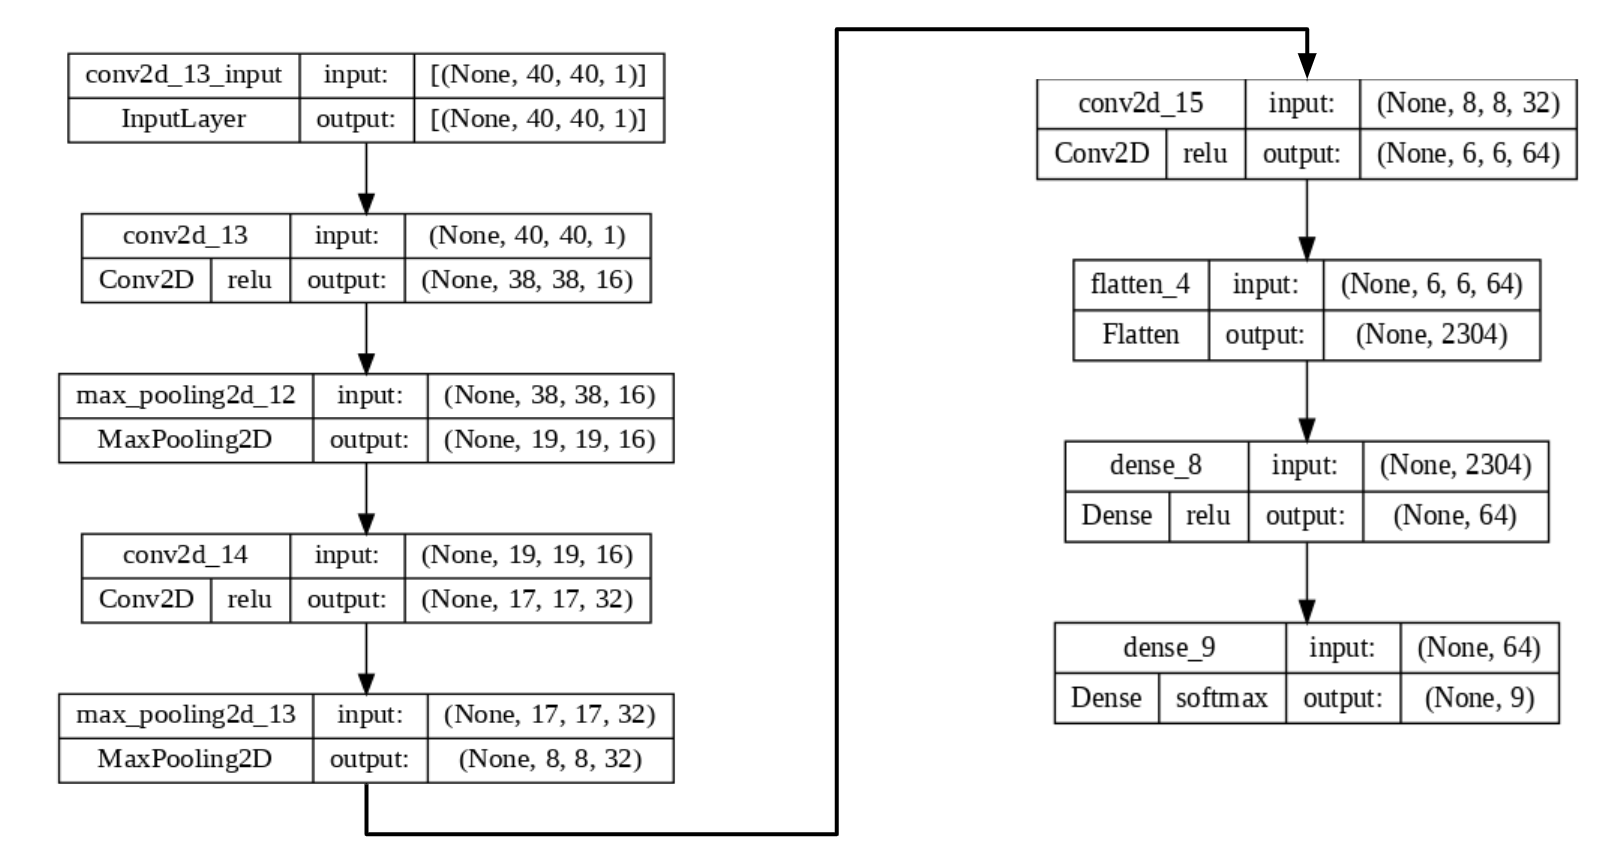
\includegraphics[width=0.8\textwidth]{Images/Perf_Eval/NN_Architecture.png}
    \caption{CNN\_Model\_1 Network Architecture}
\end{figure}

\clearpage

\section{Comparison with Model Versions}

We have two versions of our model named CNN\_Model\_0 \& CNN\_Model\_1, below are the different metrics of comparisons between our models.

\noindent The models have achieved a testing accuracy of 99\% \& 99.2\% for CNN\_Model\_0 \& CNN\_Model\_1 respectively. For an in-depth comparison, Table 4.1 is useful as we can see that class 3 of CNN\_Model\_0 has a little dip while in the figure of CNN\_Model\_1, the model has learned all classes equally.

\noindent Comparing the confusion matrices (given in Table 4.2), CNN\_Model\_0 showed a slight dip in accuracy for classes 3 \& 5, indicating room for improvement. In contrast, CNN\_Model\_1 demonstrated balanced learning across all classes, indicating its ability to classify instances accurately. These insights guide us in refining our models for enhanced performance and accuracy.

\noindent The data, given in Table 4.3, compare the performance metrics for the two versions of CNN models. We can see that the precision values have not changed with the change in versions. But the recall values have decreased by 0.001 to reach 0.986 in CNN\_ Model\_1. Also, the F1-scores have decreased by 0.011 to reach 0.988 in CNN\_ Model\_1.

\begin{table}[h!]
    \centering
    \caption{Accuracy By Class Comparison CNN\_Model\_0 \& CNN\_Model\_1}
    \begin{tabular}{|c|c|}
      \hline
      \textbf{CNN\_Model\_0} & \textbf{CNN\_Model\_1} \\
      \hline
      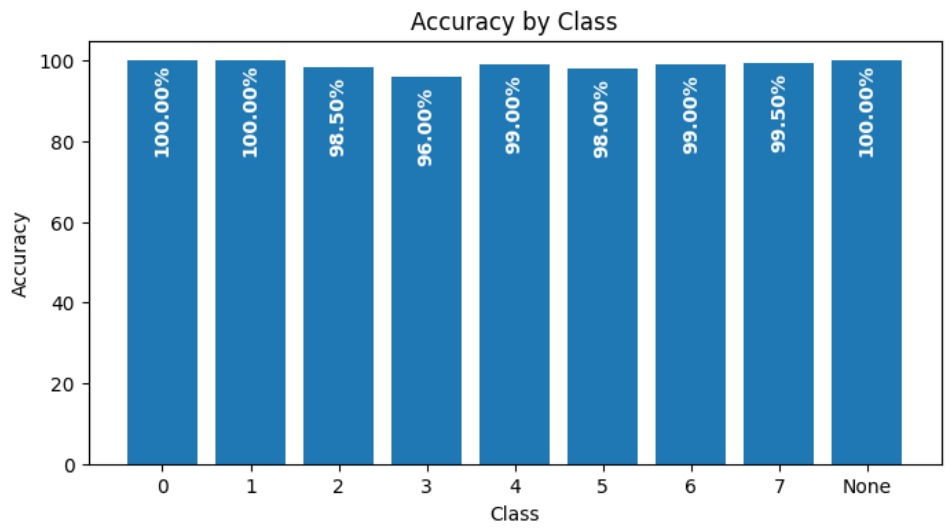
\includegraphics[width=0.5\textwidth]{Images/Perf_Eval/M0_acc_by_cls.png} & 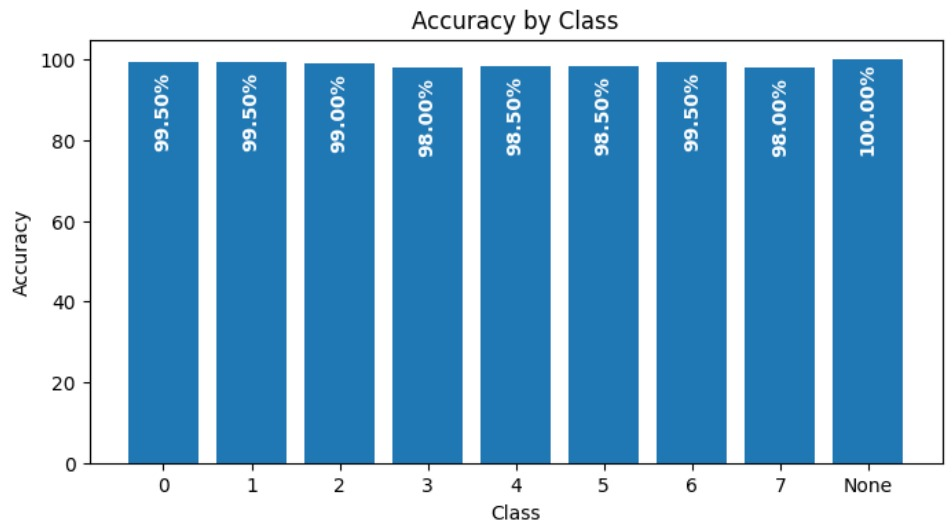
\includegraphics[width=0.5\textwidth]{Images/Perf_Eval/M1_acc_by_cls.png} \\
      \hline
    \end{tabular}
\end{table}

\begin{table}[h!]
    \centering
    \caption{Confusion Matrix Comparison CNN\_Model\_0 \& CNN\_Model\_1}
    \begin{tabular}{|c|c|}
      \hline
      \textbf{CNN\_Model\_0} & \textbf{CNN\_Model\_1} \\
      \hline
      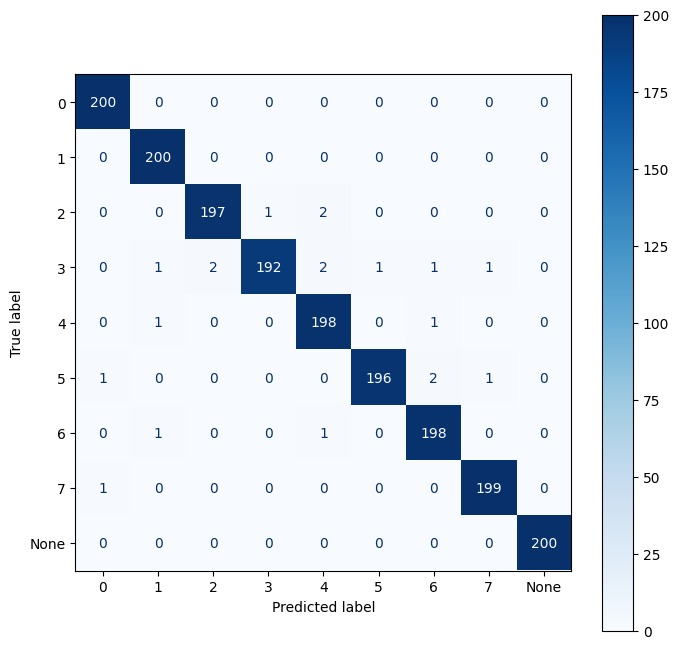
\includegraphics[width=0.5\textwidth]{Images/Perf_Eval/M0_Conf_mat.jpg} & 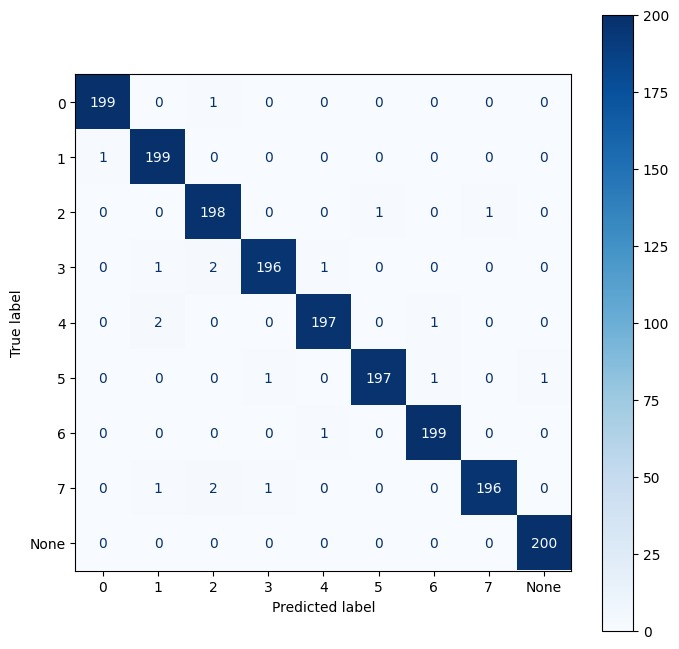
\includegraphics[width=0.5\textwidth]{Images/Perf_Eval/M1_Conf_mat.png} \\
      \hline
    \end{tabular}
\end{table}

\begin{table}[h!]
  \centering
  \caption{Performance metrics comparison for two versions of CNN Models}
  \begin{tabular}{|c|c|c|c|c|c|c|c|c|c|c|}
  \hline
   & 0 & 1 & 2 & 3 & 4 & 5 & 6 & 7 & \text{None} & \text{Overall} \\ \hline
  \multicolumn{11}{|c|}{\text{CNN\_Model\_0}} \\ \hline
  \text{Precision} & 0.99 & 0.99 & 0.99 & 0.99 & 0.98 & 0.99 & 0.98 & 0.99 & 1 & 0.988 \\ \hline
  \text{Recall} & 1 & 1 & 0.98 & 0.96 & 0.99 & 0.98 & 0.99 & 0.99 & 1 & 0.987 \\ \hline
  \text{F1-Score} & 1 & 0.99 & 0.99 & 0.98 & 0.98 & 0.99 & 0.99 & 0.99 & 1 & 0.999 \\ \hline
  \multicolumn{11}{|c|}{\text{CNN\_Model\_1}} \\ \hline
  \text{Precision} & 0.99 & 0.98 & 0.98 & 0.99 & 0.99 & 0.99 & 0.99 & 0.99 & 1 & 0.988 \\ \hline
  \text{Recall} & 0.99 & 0.99 & 0.99 & 0.98 & 0.98 & 0.98 & 0.99 & 0.98 & 1 & 0.986 \\ \hline
  \text{F1-Score} & 0.99 & 0.99 & 0.98 & 0.98 & 0.99 & 0.99 & 0.99 & 0.99 & 1 & 0.988 \\ \hline
  \end{tabular}
\end{table}

\clearpage

\section{Comparison with State-of-the-Art Methods}

% \vspace{0.3 cm}

The Marks2CSV application utilizes a cutting-edge CNN model developed from scratch, incorporating diverse libraries and modern techniques. This model represents a significant advancement in accuracy, precision, and recall (see Figure 4.6), and can even outperform previous state-of-the-art technologies.

\noindent One key advantage of the Marks2CSV application is its exceptional efficiency, providing outputs within seconds. The output is in CSV format, which is both machine-readable and writable, allowing seamless integration with existing data processing workflows. This time-saving capability and data manipulability distinguish Marks2CSV from other tools, making it invaluable for various applications.

\noindent The LeNet5 model, on the other hand, serves the specific purpose of detecting numerical and mathematical operations. While sharing a similar architecture with our CNN model, the divergent outcomes arise from their distinct task focus.

\begin{figure}[htbp]
  \centering

  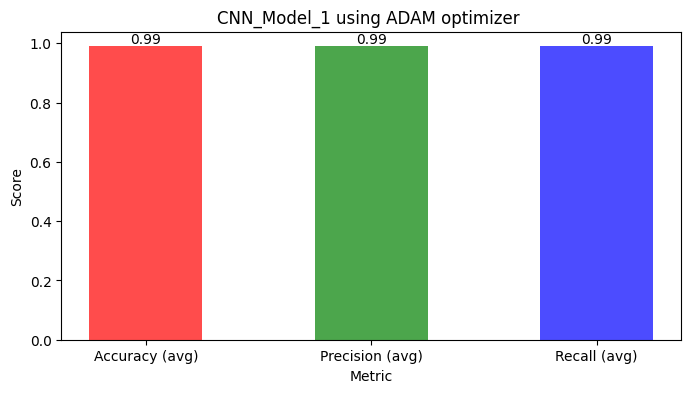
\includegraphics[width=0.45\textwidth]{Images/Results_Discussions/CNN_Model_1 ADAM.png}
  \hfill
  \subfigure{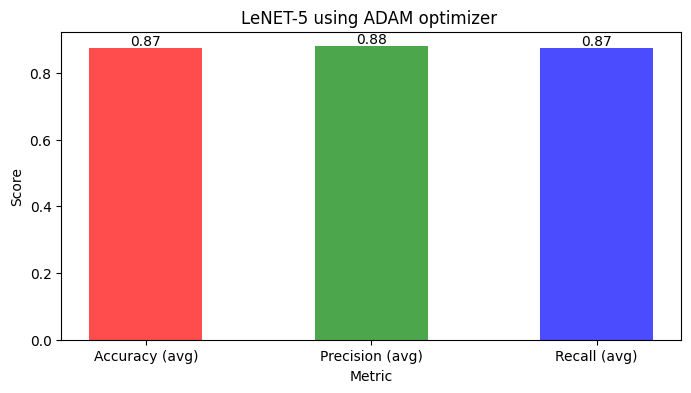
\includegraphics[width=0.45\textwidth]{Images/Results_Discussions/Lanet5 ADAM.png}}
  \caption{Model Comparison: Our Model vs LeNet5 with ADAM Optimizer}

  \vspace{0.5cm} % Adjust the vertical spacing between the rows of images

  \subfigure{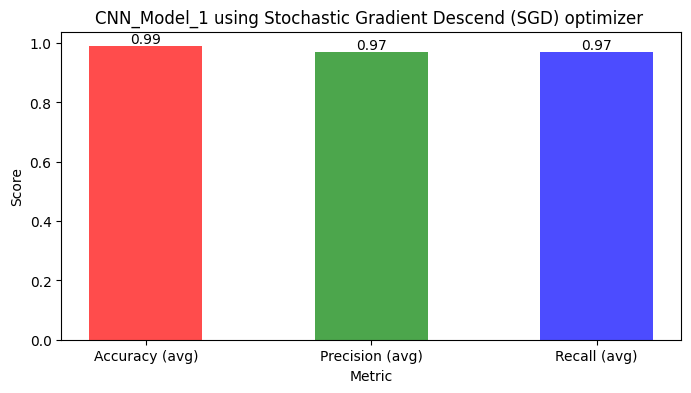
\includegraphics[width=0.45\textwidth]{Images/Results_Discussions/CNN_Model_1 SGD.png}}
  \hfill
  \subfigure{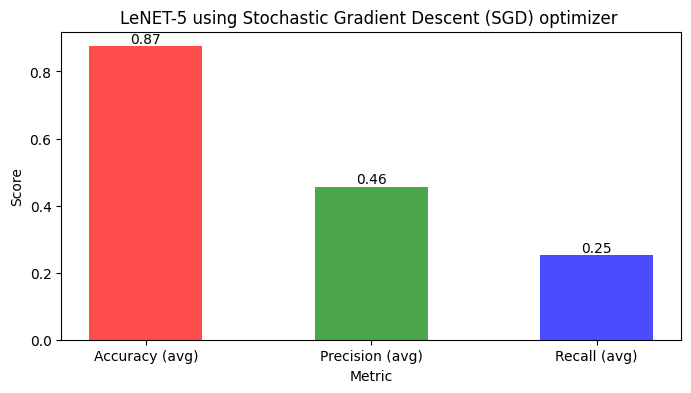
\includegraphics[width=0.45\textwidth]{Images/Results_Discussions/Lanet5 SGD.png}}
  \caption{Model Comparison: Our Model vs LeNet5 with SGD Optimizer}
  
\end{figure}

\clearpage

\section{Discussion}

In the evaluation of two models, namely CNN-Model-1 and LeNet5, their performance was analyzed using two different optimizers: Adam and SGD. The objective was to assess the impact of optimizer choice on the models' accuracy.

\noindent When testing CNN-Model-1 with both Adam and SGD optimizers, it was observed that there was no significant change in accuracy. Regardless of the optimizer used, CNN-Model-1 consistently performed well, indicating its robustness and stability. This suggests that the choice of optimizer had minimal influence on the model's overall accuracy. Thus, CNN-Model-1 demonstrated its superiority by consistently maintaining a high level of accuracy in both optimizer scenarios.

\noindent On the other hand, LeNet5 exhibited a contrasting behavior when tested with Adam and SGD optimizers. While LeNet5 initially showed promising results with the Adam optimizer, a considerable performance drop was observed when switching to the SGD optimizer. This performance degradation indicates that the SGD optimizer was not suitable for the LeNet5 architecture, leading to a significant decrease in accuracy. This discrepancy highlights the sensitivity of LeNet5 to the choice of optimizer and emphasizes the importance of selecting an appropriate optimizer for optimal performance.

\noindent Based on these findings, it is evident that CNN-Model-1 outperformed LeNet5 in both optimizer scenarios. CNN-Model-1 consistently demonstrated higher accuracy and showcased its robustness by maintaining its superior performance regardless of the optimizer choice. These results emphasize the effectiveness and superiority of CNN-Model-1 over LeNet5, positioning it as a more reliable and accurate model for the given task.

\noindent It is worth noting that further analysis and experimentation may be required to determine the underlying factors contributing to the contrasting performances of the two models with different optimizers. Additional investigations into model architecture, dataset characteristics, and hyperparameter tuning could provide valuable insights into the observed performance differences.

% \end{document}